% Compile with XeLaTeX on Overleaf.
\documentclass[11pt,a4paper]{article}

\usepackage[UTF8]{ctex}
\usepackage[a4paper,margin=1in]{geometry}
\usepackage{graphicx}
\usepackage{booktabs}
\usepackage{float}
\usepackage{hyperref}
\usepackage{amsmath}
\usepackage{array}

\hypersetup{
    colorlinks=true,
    linkcolor=blue,
    urlcolor=blue,
    citecolor=blue
}

\newcommand{\githuburl}{\url{https://github.com/highevolutionary/Project-2-of-Neural-Network-and-Deep-Learning.git}}
\newcommand{\dataseturl}{\url{https://www.cs.toronto.edu/~kriz/cifar.html}}

\title{Project-2 of ``Neural Network and Deep Learning''}
\author{李星 \\ Student ID: 22300290002}
\date{\today}

\begin{document}
\maketitle

\begin{abstract}
This report studies image classification on CIFAR-10 and Batch Normalization in
VGG-A. The first part trains a compact convolutional network with residual
blocks, squeeze-and-excitation modules, Batch Normalization, dropout, and data
augmentation. I compare different activations, model structures, regularization
strengths, and optimizers while changing only one variable at a time. The best
test accuracy in this part is 88.91\%. The second part compares VGG-A with and
without Batch Normalization and visualizes the loss landscape. All code files,
training scripts, figures, tables, and trained model weights are available in
the GitHub repository: \githuburl.
\end{abstract}

\section{Train a Network on CIFAR-10}

\subsection{Methodology}

\subsubsection{Data Augmentation}

CIFAR-10 contains 50,000 training images and 10,000 test images from 10 classes.
The dataset link is \dataseturl. I used the full training set and the official
test batch, without creating an extra validation split. Training samples were
augmented by random crop, horizontal flip, and color jitter. Test images were
only normalized.

\begin{table}[H]
\centering
\caption{Main hyperparameter settings for the CIFAR-10 classification network.}
\begin{tabular}{ll}
\toprule
Hyperparameter & Setting \\
\midrule
Train batch size & 192 \\
Test batch size & 384 \\
Random crop & padding=3, padding mode=reflect \\
Color jitter & brightness=0.25, contrast=0.25, saturation=0.25, hue=0.10 \\
Normalization mean & (0.4915, 0.4823, 0.4468) \\
Normalization std & (0.2023, 0.1994, 0.2010) \\
Loss function & Cross-Entropy \\
Default activation & ReLU \\
Weight initialization & Kaiming Normal for ReLU, Xavier Uniform for Tanh/Sigmoid \\
Dropout & Normal dropout, rate=0.4 \\
Optimizer & Adam \\
Maximum learning rate & 0.0008 \\
Weight decay & 0.0003 \\
Gradient clipping & 0.8 \\
Early stopping & patience=16, min delta=0.0007 \\
\bottomrule
\end{tabular}
\end{table}

The numerical settings are chosen independently for this experiment, while the
experiment categories follow the project requirements: structure, activation,
loss/regularization, and optimizer comparisons.

\subsubsection{Model Structure}

The main network is a compact CNN designed for CIFAR-10. It starts with a
$5\times5$ stem convolution that maps RGB input to 24 channels. The feature
extractor contains three stages. The channel widths are 24, 32, and 64. Each
stage contains repeated residual basic blocks. Each basic block uses two
convolutional layers, Batch Normalization, an activation function, a residual
shortcut, and a squeeze-and-excitation module. The final representation is
obtained by adaptive average pooling and passed to a fully connected classifier
with 128 hidden units, dropout, and a final 10-way linear layer.

This architecture contains the required components: fully connected layers,
2D convolutional layers, 2D pooling through adaptive average pooling, activation
functions, Batch Normalization, dropout, and residual connections.

\subsubsection{Training Procedure}

The model is trained with cross entropy loss and a warmup-cosine learning-rate
schedule. The learning rate increases linearly during warmup and then follows a
cosine decay. After warmup, gradient norms are clipped to 0.8. At the end of
each epoch, the model is evaluated on the CIFAR-10 test batch. The log reports
both training accuracy and test accuracy.

\subsection{Experiments}

\subsubsection{Insights}

The baseline network uses ReLU, 6 blocks per stage, Adam, learning rate 0.0008,
weight decay 0.0003, and dropout 0.4. It has 629,766 trainable parameters and
achieves 88.42\% best test accuracy.

\begin{table}[H]
\centering
\caption{Baseline result.}
\begin{tabular}{lrrrr}
\toprule
Experiment & Parameters & Best Test Acc. & Best Epoch & Final Test Acc. \\
\midrule
Baseline & 629,766 & 88.42\% & 47 & 88.35\% \\
\bottomrule
\end{tabular}
\end{table}

\begin{figure}[H]
\centering
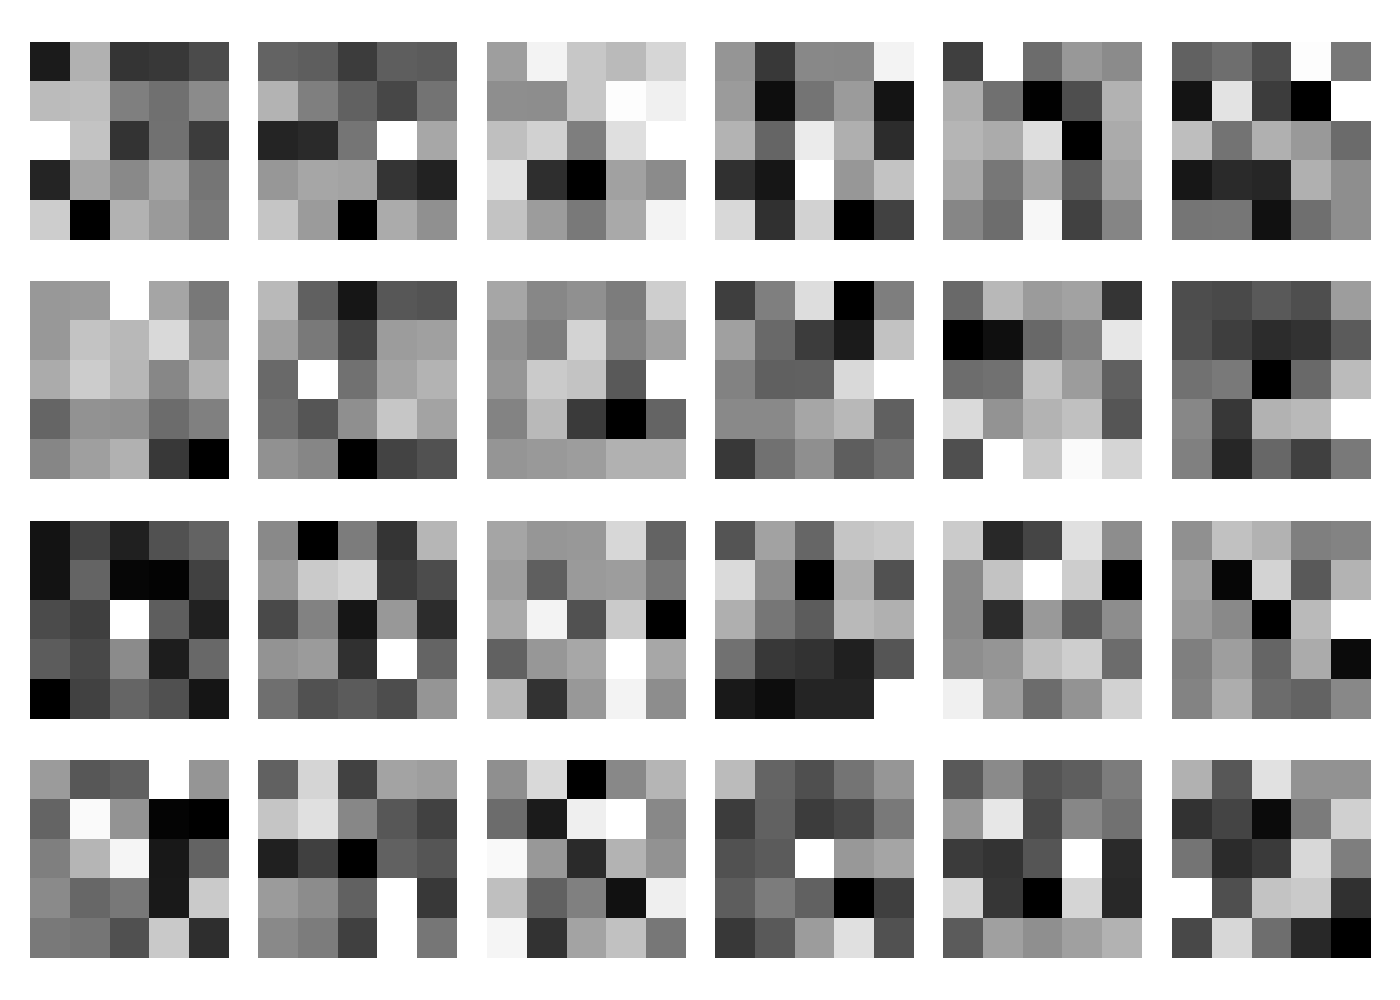
\includegraphics[width=0.72\linewidth]{figures/first_layer_filters.png}
\caption{Visualization of the first-layer convolutional filters.}
\end{figure}

The first-layer filters show low-level visual patterns such as edge-like and
contrast-sensitive responses. This provides a simple interpretation of what the
network learns at the earliest stage.

\subsubsection{Different Activation}

For the activation comparison, only the activation function is changed. All
other settings are kept the same as the baseline.

\begin{table}[H]
\centering
\caption{Activation comparison.}
\begin{tabular}{lrrr}
\toprule
Activation & Parameters & Best Test Acc. & Best Epoch \\
\midrule
ReLU & 629,766 & \textbf{88.75\%} & 48 \\
Tanh & 629,766 & 83.72\% & 50 \\
Sigmoid & 629,766 & 20.76\% & 1 \\
\bottomrule
\end{tabular}
\end{table}

\begin{figure}[H]
\centering
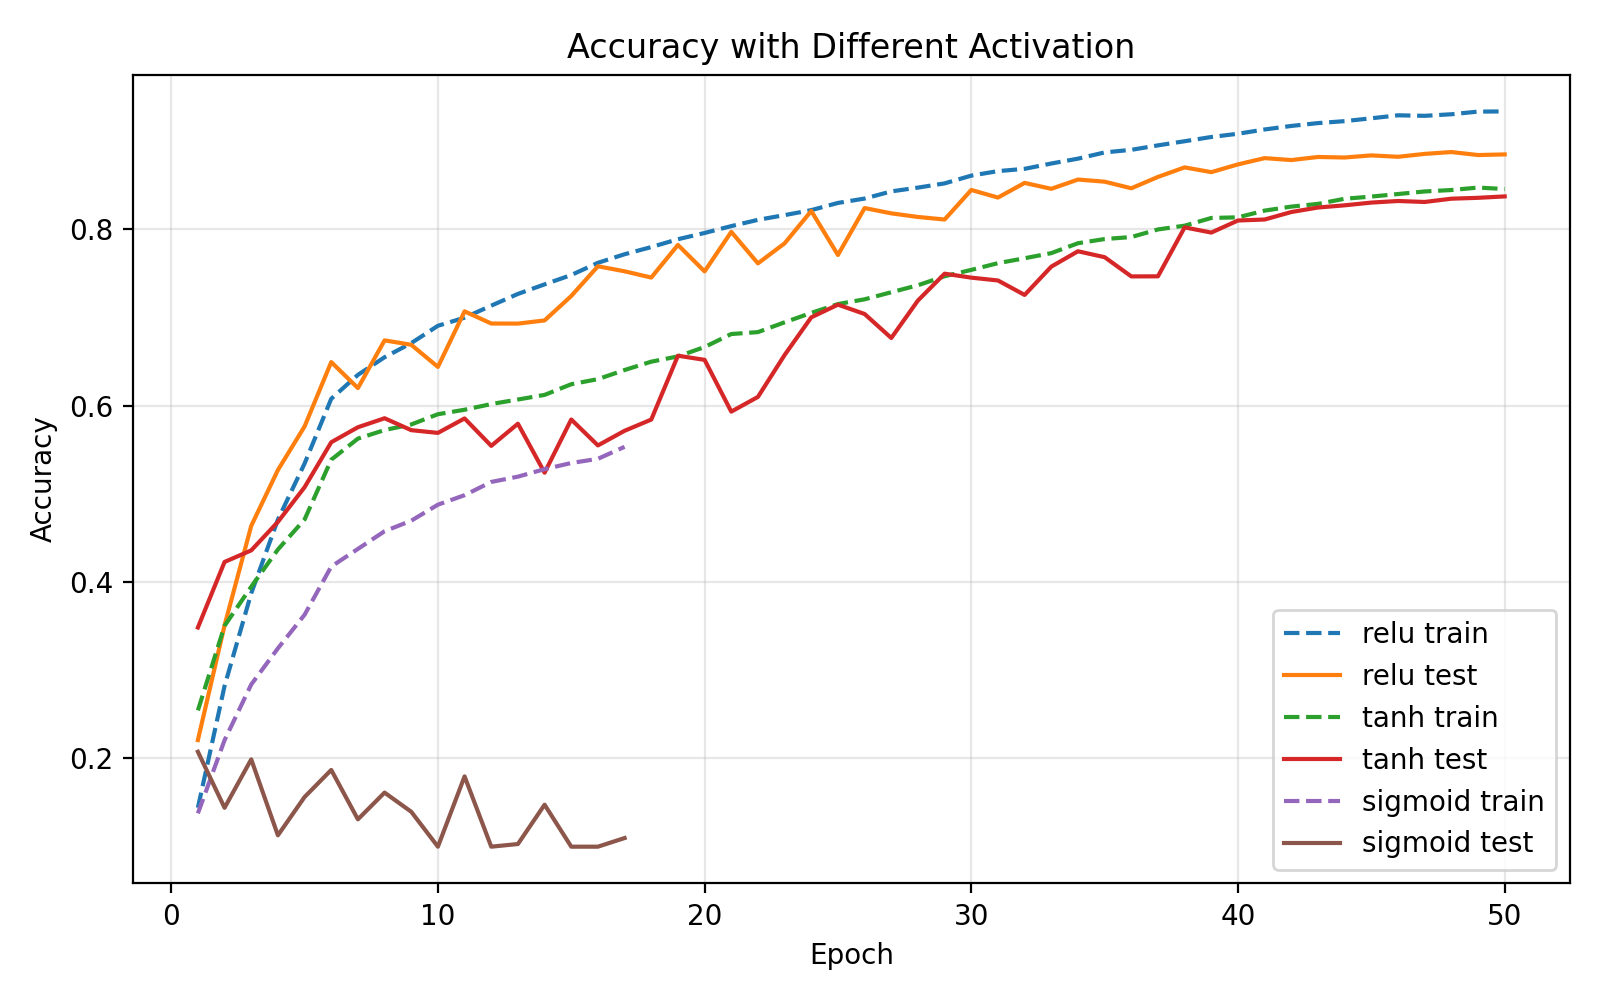
\includegraphics[width=0.90\linewidth]{figures/activation_comparison.png}
\caption{Training and testing accuracy with different activation functions.}
\end{figure}

ReLU performs best. Tanh can still train the network but converges to lower
accuracy. Sigmoid performs poorly, which is consistent with saturation and weak
gradient flow in deeper convolutional networks.

\subsubsection{Different Structure}

For the structure comparison, only the number of residual blocks in each stage
is changed. The compared settings are 5, 6, and 7 blocks per stage.

\begin{table}[H]
\centering
\caption{Structure comparison.}
\begin{tabular}{lrrr}
\toprule
Structure & Parameters & Best Test Acc. & Best Epoch \\
\midrule
5 blocks/stage & 523,760 & \textbf{88.91\%} & 47 \\
6 blocks/stage & 629,766 & 88.31\% & 48 \\
7 blocks/stage & 735,772 & 88.09\% & 49 \\
\bottomrule
\end{tabular}
\end{table}

\begin{figure}[H]
\centering
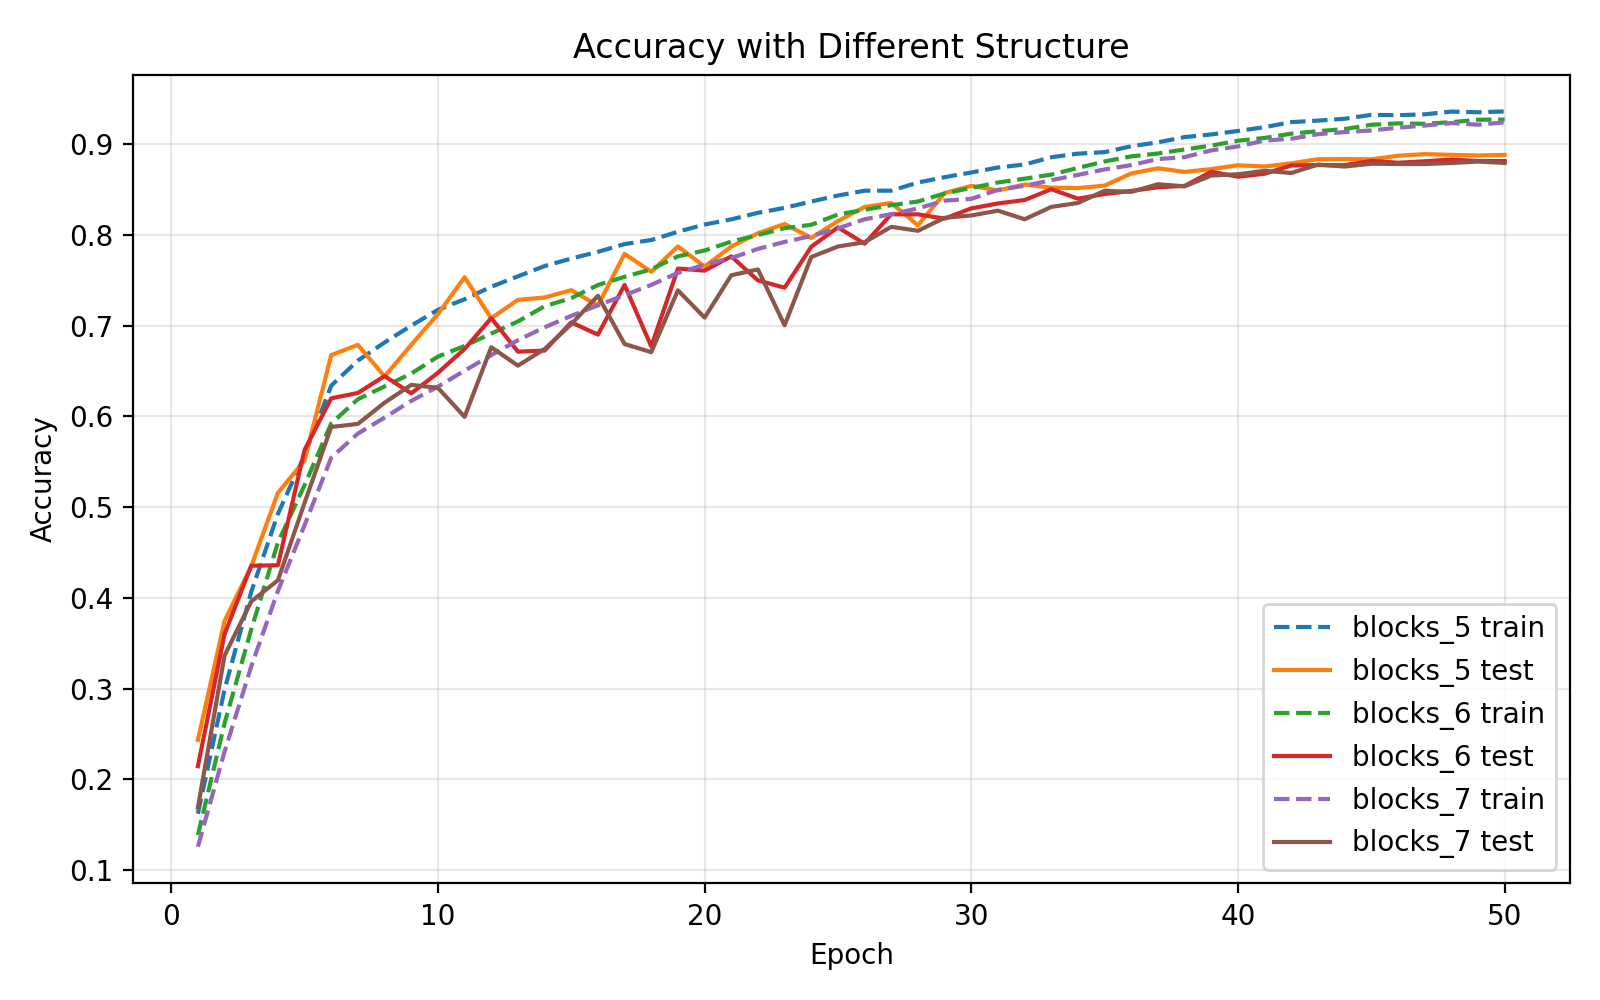
\includegraphics[width=0.90\linewidth]{figures/structure_comparison.png}
\caption{Training and testing accuracy with different model structures.}
\end{figure}

Increasing the number of blocks does not always improve test accuracy. In this
run, the 5-block structure is slightly better while also using fewer parameters,
suggesting that the deeper variants may be harder to optimize or slightly
over-parameterized for this setting.

\subsubsection{Different Loss and Regularization}

The loss function remains cross entropy, while the regularization strength is
changed through weight decay. This changes only the regularization term.

\begin{table}[H]
\centering
\caption{Loss/regularization comparison.}
\begin{tabular}{lrrr}
\toprule
Weight Decay & Parameters & Best Test Acc. & Best Epoch \\
\midrule
$5\times10^{-5}$ & 629,766 & 87.68\% & 45 \\
$3\times10^{-4}$ & 629,766 & 88.39\% & 50 \\
$8\times10^{-4}$ & 629,766 & \textbf{88.72\%} & 48 \\
\bottomrule
\end{tabular}
\end{table}

\begin{figure}[H]
\centering
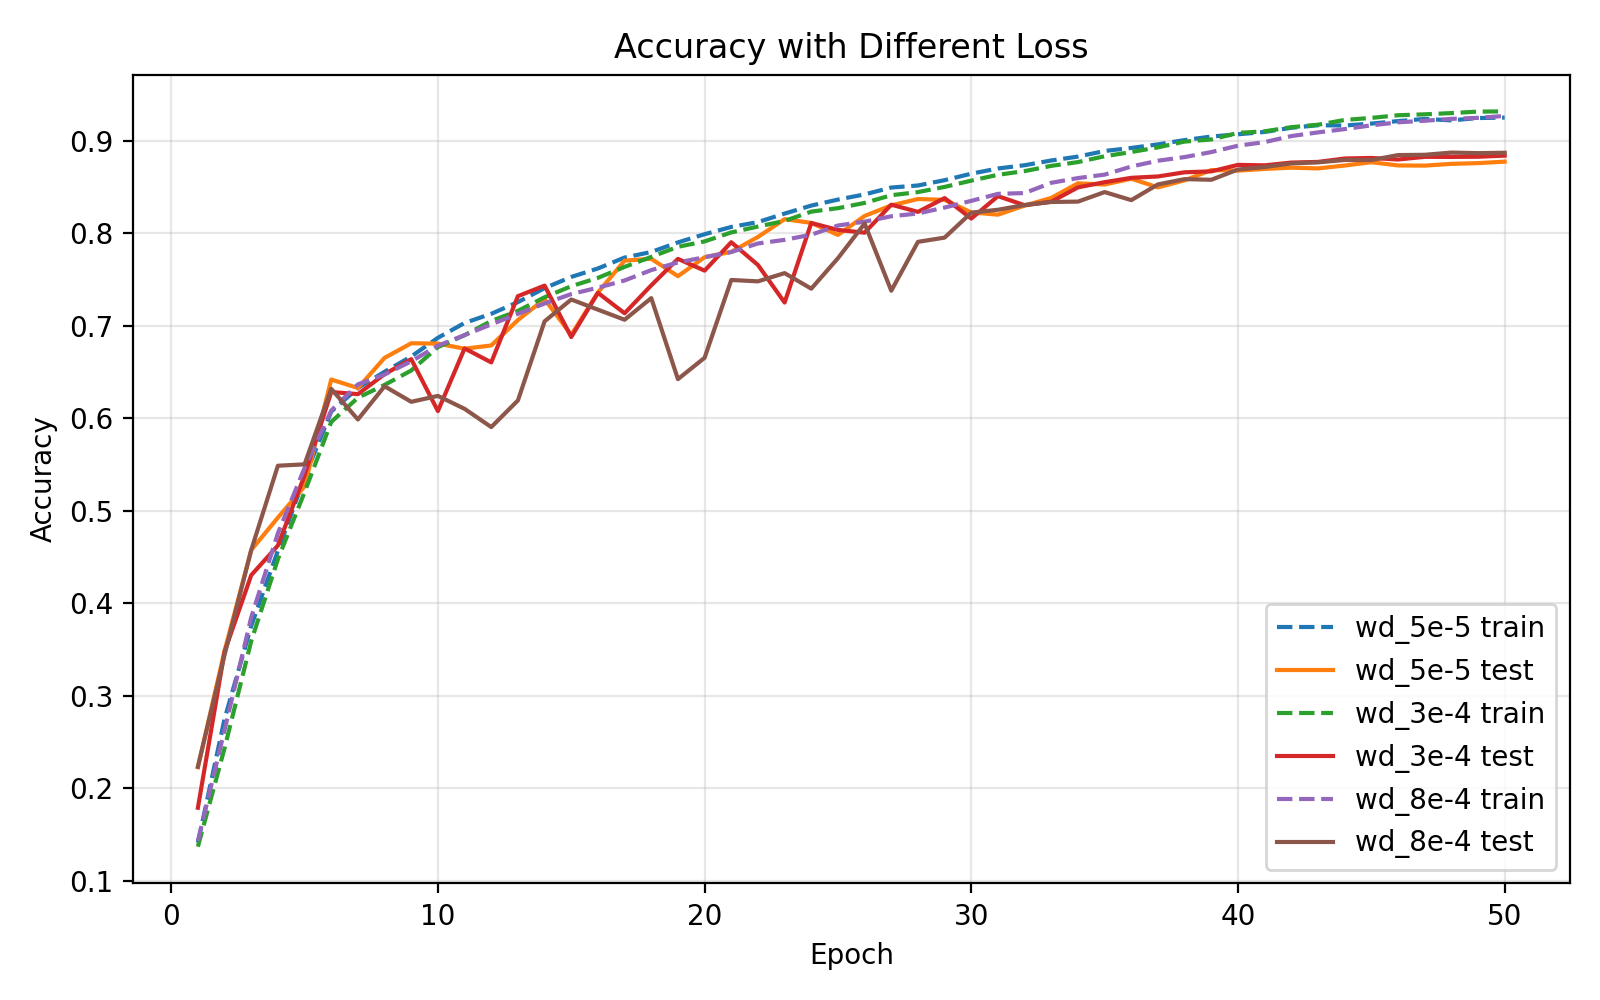
\includegraphics[width=0.90\linewidth]{figures/loss_comparison.png}
\caption{Training and testing accuracy with different regularization settings.}
\end{figure}

Moderate to stronger weight decay improves generalization in this setting. The
best regularization result is obtained with weight decay $8\times10^{-4}$.

\subsubsection{Different Optimizer}

For the optimizer comparison, only the optimizer is changed. I compare Adam and
SGD with momentum using the same maximum learning rate and weight decay.

\begin{table}[H]
\centering
\caption{Optimizer comparison.}
\begin{tabular}{lrrr}
\toprule
Optimizer & Parameters & Best Test Acc. & Best Epoch \\
\midrule
Adam & 629,766 & \textbf{88.39\%} & 50 \\
SGD & 629,766 & 30.85\% & 47 \\
\bottomrule
\end{tabular}
\end{table}

\begin{figure}[H]
\centering
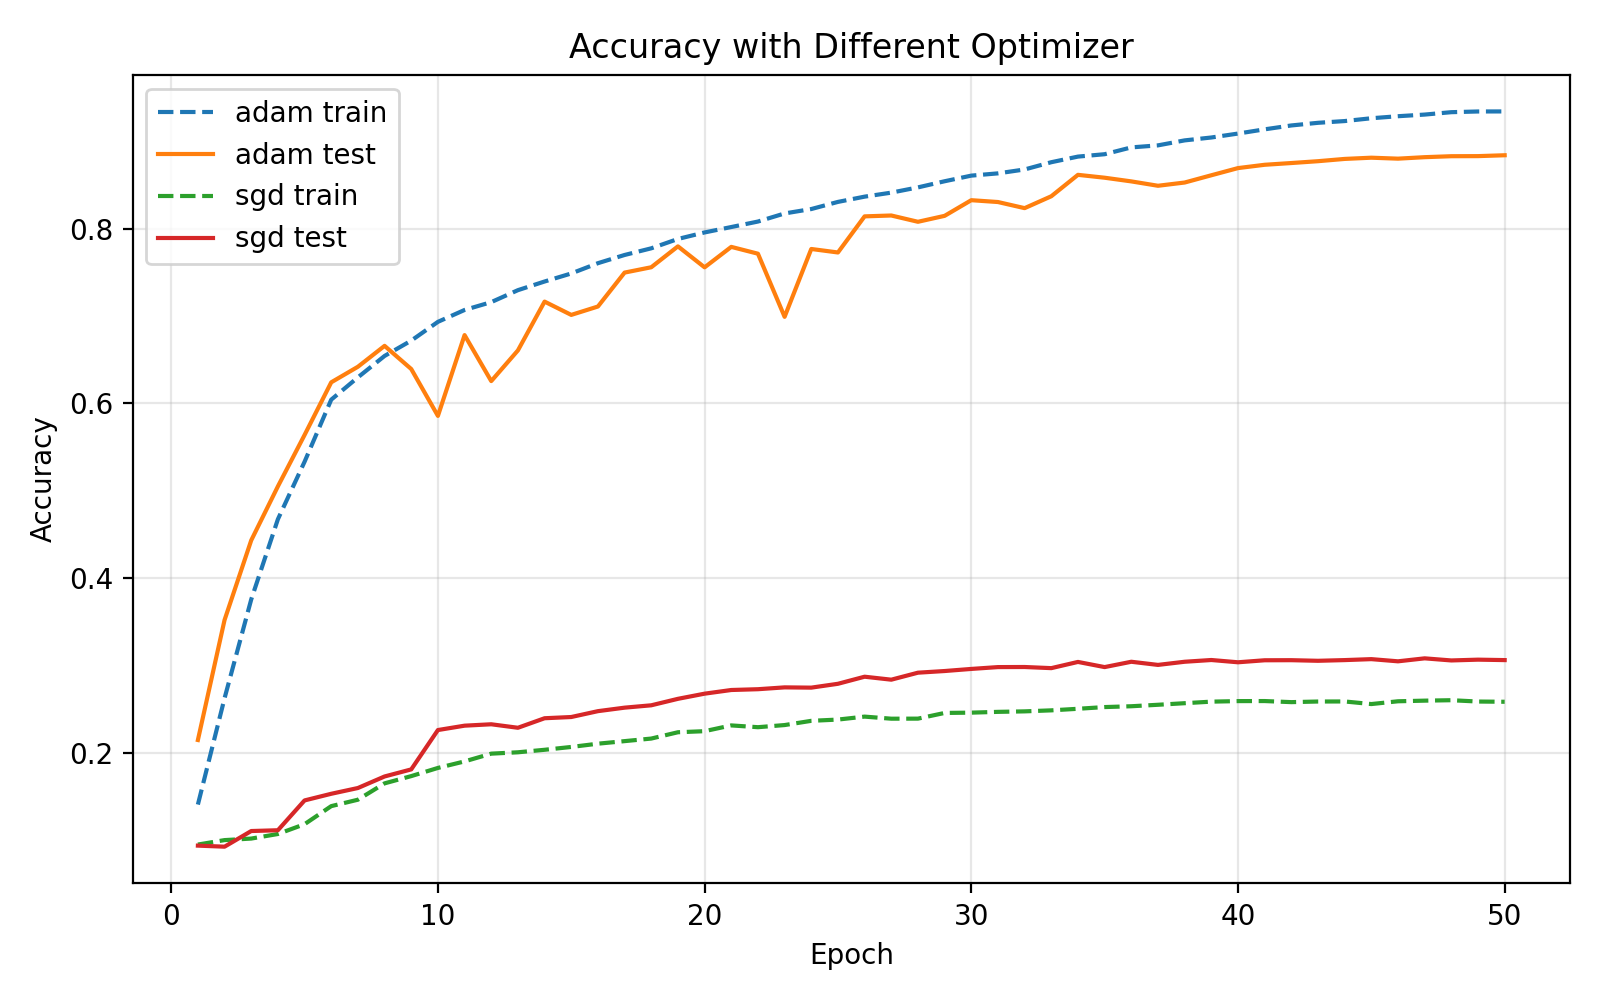
\includegraphics[width=0.90\linewidth]{figures/optimizer_comparison.png}
\caption{Training and testing accuracy with different optimizers.}
\end{figure}

Adam converges much faster under the selected learning-rate scale. SGD performs
poorly here, indicating that it would require a different learning-rate setting
or a longer schedule to be competitive.

\section{Batch Normalization}

Batch Normalization normalizes intermediate activations and learns channel-wise
scale and shift parameters. In this part, I compare VGG-A with and without BN.
The BN version adds a BatchNorm2d layer after each convolutional layer.

\subsection{Training Process Comparison}

The VGG-A experiments use Adam, cross entropy, 20 epochs, and the same CIFAR-10
train/test split. Four learning rates are tested to satisfy the loss-landscape
requirement.

\begin{table}[H]
\centering
\caption{VGG-A and VGG-A-BN comparison.}
\begin{tabular}{lrrr}
\toprule
Model & Learning Rate & Parameters & Best Test Acc. \\
\midrule
VGG-A & 0.001 & 9,750,922 & 81.66\% \\
VGG-A & 0.002 & 9,750,922 & 78.20\% \\
VGG-A & 0.0001 & 9,750,922 & 77.95\% \\
VGG-A & 0.0005 & 9,750,922 & 83.31\% \\
VGG-A-BN & 0.001 & 9,756,426 & 86.88\% \\
VGG-A-BN & 0.002 & 9,756,426 & \textbf{87.27\%} \\
VGG-A-BN & 0.0001 & 9,756,426 & 81.07\% \\
VGG-A-BN & 0.0005 & 9,756,426 & 85.70\% \\
\bottomrule
\end{tabular}
\end{table}

\begin{figure}[H]
\centering
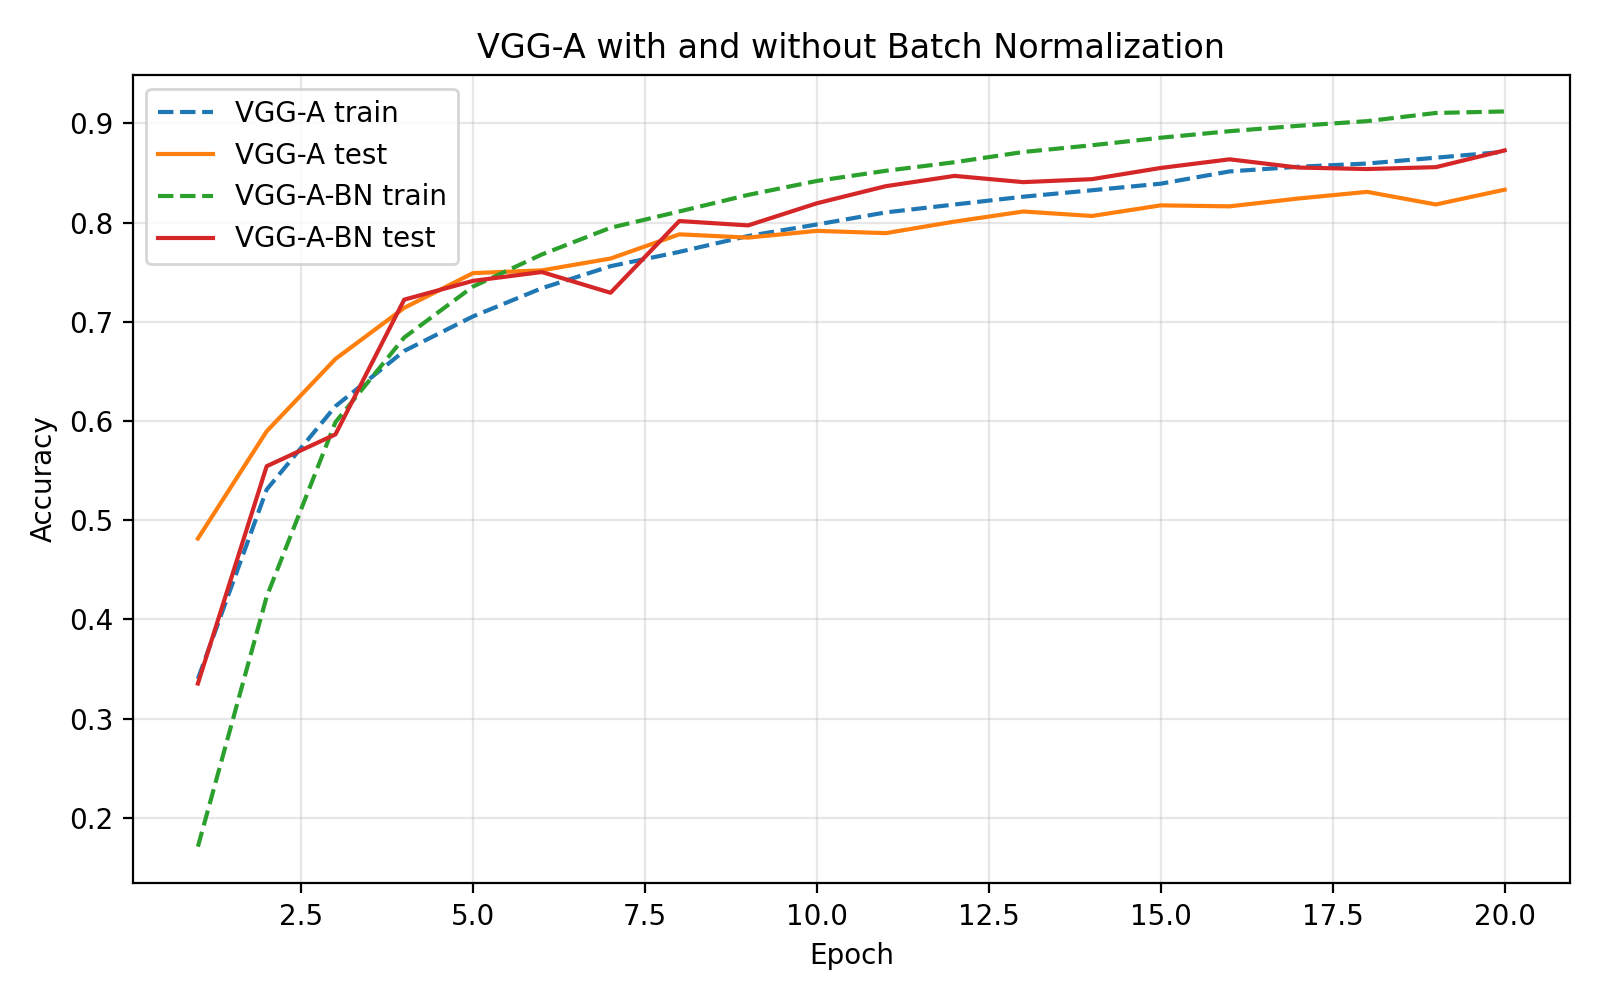
\includegraphics[width=0.90\linewidth]{figures/vgg_bn_training_comparison.png}
\caption{Training and testing accuracy for VGG-A with and without BN.}
\end{figure}

The best VGG-A-BN accuracy is 87.27\%, while the best VGG-A accuracy is 83.31\%.
BN improves the best test accuracy by 3.96 percentage points and is especially
helpful at larger learning rates.

\subsection{Loss Landscape Comparison}

Following the project instruction, I train multiple VGG-A and VGG-A-BN models
with learning rates $10^{-3}$, $2\times10^{-3}$, $10^{-4}$, and
$5\times10^{-4}$. For each training step, I collect the losses from all
learning-rate runs, compute the minimum and maximum curves, and fill the region
between them using \texttt{matplotlib.pyplot.fill\_between}.

\begin{figure}[H]
\centering
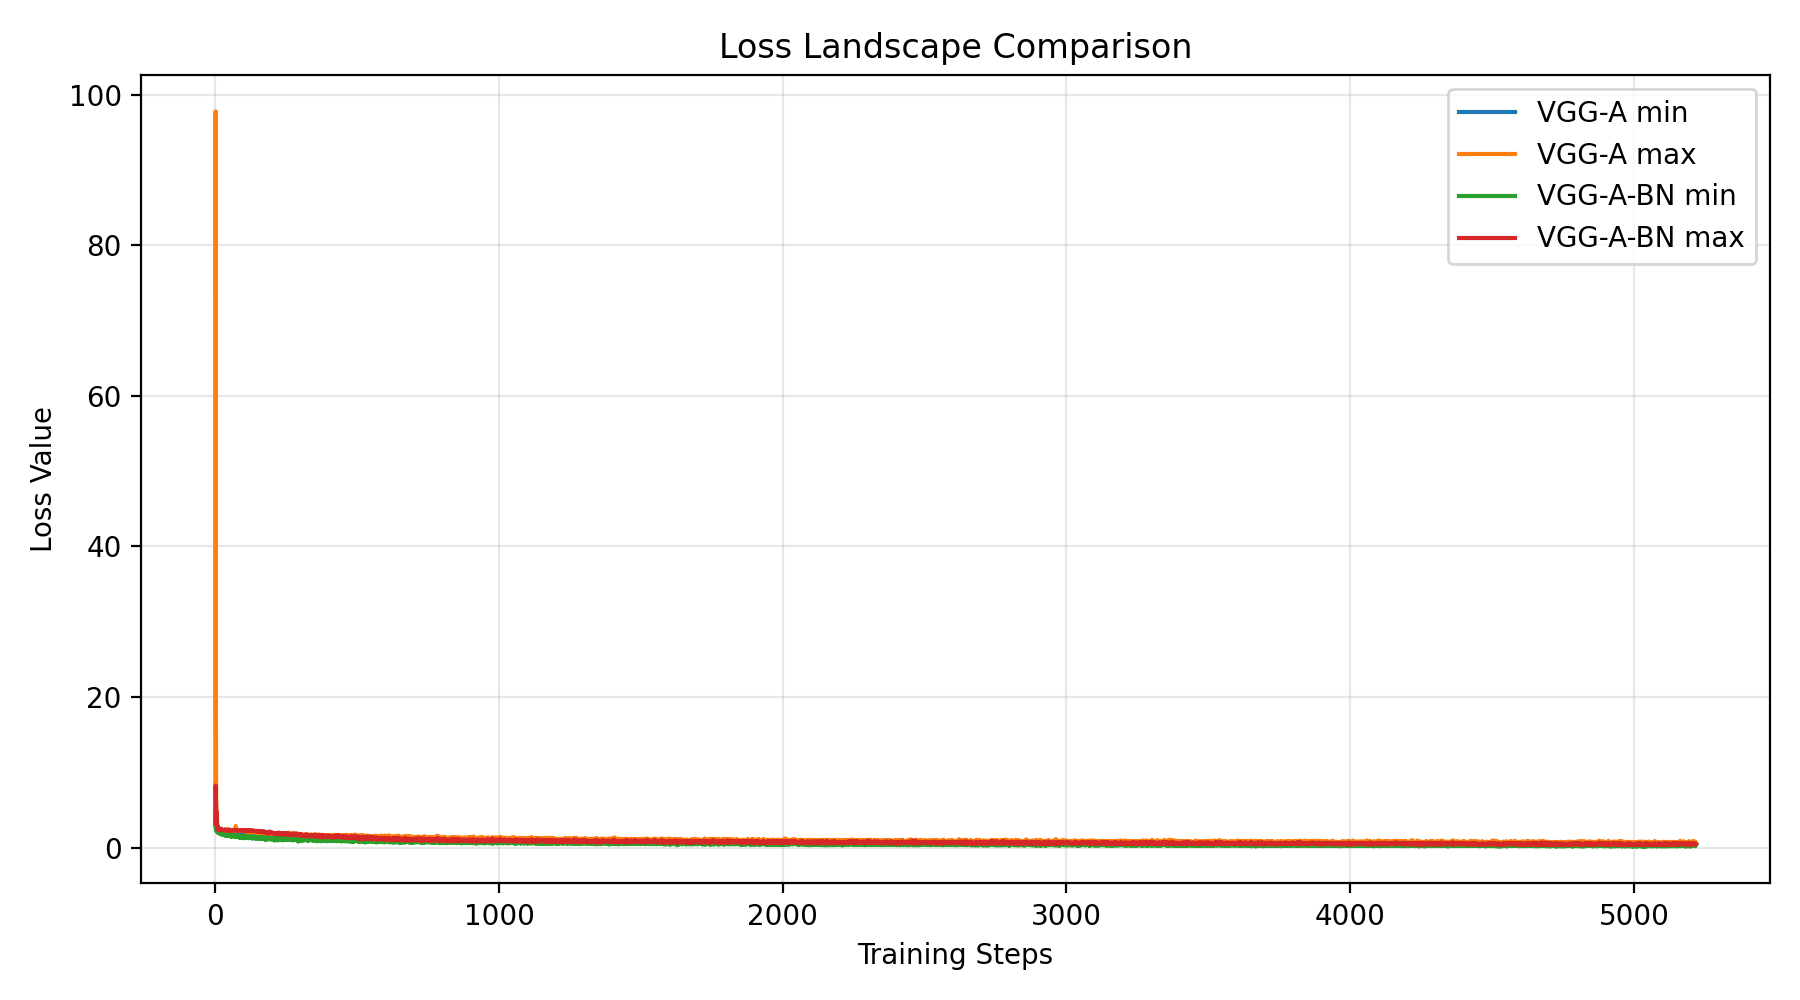
\includegraphics[width=0.90\linewidth]{figures/vgg_loss_landscape_comparison.png}
\caption{Loss landscape comparison of VGG-A and VGG-A-BN.}
\end{figure}

The BN model has lower and more stable loss behavior across learning rates. This
visualization supports the interpretation that BN smooths the optimization
process and reduces sensitivity to the choice of step size.

\section{Conclusion}

The compact residual CNN achieves 88.91\% best test accuracy with 5 blocks per
stage and 523,760 parameters. The controlled experiments show that ReLU is the
best activation among the tested choices, moderate weight decay improves
generalization, and Adam is much more effective than SGD under the selected
settings. For the VGG-A study, Batch Normalization improves the best test
accuracy from 83.31\% to 87.27\% and produces a smoother loss landscape. These
results satisfy the project requirements on CIFAR-10 training, optimization
comparison, BN comparison, and model interpretation.

\appendix
\section{Reproducibility}

The main command used on the GPU server was:
\begin{verbatim}
nohup python run_reworked_project2.py --device cuda:0 > train_reworked.log 2>&1 &
\end{verbatim}

The output files used in this report are:
\begin{itemize}
    \item \texttt{pj2\_reworked\_outputs/tables/course\_cnn\_summary.csv}
    \item \texttt{pj2\_reworked\_outputs/tables/vgg\_bn\_summary.csv}
    \item \texttt{pj2\_reworked\_outputs/figures/*.png}
    \item \texttt{pj2\_reworked\_outputs/models/*.pt}
\end{itemize}

\end{document}
